\section{Implementering}
I dette afsnit vil implementeringen af systemet blive gennemgået, både hvordan det funktionelle er skruet sammen, men også de brugergrænseflader der omfavner det hele. Nogle af de kriterier der skal være opfyldt for at kunne implementere systemet, vil også blive forklaret.

\subsection{Kriterier for socialt medie}
\label{Kriterier_Medie}
Et kritisk komponent af systemet er det sociale medie, som anvendes til opslag af billeder indeholdende skjulte beskeder. Dette er væsentligt at omtale af flere grunde. I det lange løb vil det være vigtigt at vælge et socialt medie, der tillader automatisk generering af anonyme brugere, da dette er essentielt i systemet. Men da det muligvis ikke er muligt at finde et sådant medie, kunne det dog være nødvendigt at nøjes med et socialt medie, der blot er langsomt til at lukke bots. Kortsigtet funktionalitet er dog endnu mere afhængigt af hvordan det enkelte medie håndterer billeder. Med dette forstås ting såsom størrelsesbegrænsninger, komprimering og formatering. Hvis et socialt medie formaterer alle billeder, uanset størrelse og filtype, vil det give flere udfordringer i hvordan systemet så kan gemme beskeder i billedet, uden at de bliver fjernet i formateringen. Dernæst er det også vigtigt at den sociale medie platform tillader kontrol over metadata. Alle disse ting skal være tilgængelige igennem et API [Forklaret i \ref{API}], for at systemet kan udføre disse opgaver automatisk.\\
Det viser sig at Instagram opfylder alle disse krav, da de ikke laver nogen formatering af billeder med en bredde imellem 320 og 1080 pixels.\cite{Instagram_Photo_Resolution}\cite{Instagram_Image_Compression} Instagram tilbyder også et API, der tillader tilføjelse af metadata. På grund af disse faktum, er Instagram valgt som det sociale medie til "proof of concept" implementation. Man kunne forestille sig, at mange andre sociale medier kunne anvendes i stedet, men dette ville kræve, at man vidste hvilke kriterier billederne skal holde sig indenfor, for at undgå formatering. Alternativt kunne det undersøges om beskeden kunne skjules på en sådan måde, at formateringen ikke påvirker den. 
\newpage

\subsection{API, REST og Socket kommunikation}
\label{API}
De fleste tjenester opsat i dag, foruden deres givende handlinger, tilbyder mulighed for at et program automatisk kan foretage interaktion, altså uden et menneskes handlinger. En sådanne maskin interaktion siges, at anvende et API (\underline{A}pplication \underline{P}rogramming \underline{I}nterface) til at standardisere dets forventede inputs og outputs. 
API står i modsætning til UI (\underline{U}ser \underline{I}nterface), hvor et menneske interagerer med en tjeneste, og beskriver hvordan, samt hvad der skal til, for at foretage bestemte handlinger, så som f.eks. efter denne rapports idé, at uploade et billede til en given tjeneste. En API er derfor generelt nødvendig for at kunne opsætte en troværdig interaktion mellem tredje parts tjenester, og den oprindelige udbyder.\cite{WhatIsAPI}\\
"API" er i dag en alment kendt metode betegnelse, og findes derfor i et utal at forskellige versioner, typer og udgivere. F.eks. er nogle af de mest kendte Googles eget API "Google-API", eller det mere standardiserede web API "REST" (\underline{RE}presentational \underline{S}tate \underline{T}ransfer), begge ikke kun anvendt i lukkede systemer, men også generelt alment på nettet.\cite{codecademy_REST}\\
En API protokol beskriver dog kun hvordan en given data forventes formateret, og ikke hvordan en data skal leveres, derfor anvender mange tjenester også en eller anden form for Socket kommunikation til at forventningsafstemme, og sikre en data leverance. Bagsiden ved opsætning af en Socket forbindelse er dog på serversiden, at disse også kræver opsætning af en listener. En listener er en server applikation, der aktivt står og lytter efter en klient, der ønsker at oprette en kommunikation på en given port. Dette vil sige at den oprindelige tjeneste, efter opsætningen af et socket, nu har et åbent interface, og derved også en øget sikkerheds risiko. Efter opsætningen er listenerens opgave at sørge for hurtigst muligt, at sikre en åben forbindelse på en anden port, mellem denne server og klient under en ny oprettet forbindelse, da porten for listeneren igen skal være fri til den næste klient. \cite{WhatIsSocket} Selv om man ikke direkte kan undgå brugen af Socket kommunikation, ved en server til klient kommunikation, og derved generelt må acceptere denne øgede sikkerheds risiko, forefindes der dog stadig flere måder at opnå samme resultat, også uden direkte opsætning af selve socket forbindelsen, så som foreksempel HTTP-REST, Active-MQ eller Rabbit-MQ, der dog også anvender Socket kommunikation, men har almen erfaring, samt konstant bliver opdateret, til at minske den ellers øgeder sikkerheds brist.\cite{SocketAlternatives}
\newpage
\subsection{Funktionalitet}
\label{funktionalitet}
Som systemets implementation for et mindre demo produkt, der også senere vil kunne udvides med eventuelle manglende funktioner, tænkes følgende tre diagrammer til beskrivelse af platformens funktionelle anvendelse.

\subsubsection{User login}
\begin{figure}[H]
    \centering
    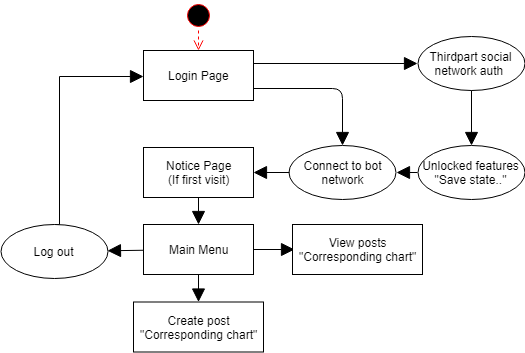
\includegraphics[width=0.60\textwidth]{Projectdoc/Assets/Illustrationer/Implementation-billede1.png}
    \label{fig:implementation1}
    \caption{Implementation 1}
\end{figure}

Gennem det 1. af 3 diagrammer bliver brugeren præsenteret for 3 views, eller sider.\\ 
Henholdsvis \textit{Login page}, hvor brugerene vil have mulighed for at indtaste deres login kriterier til deres brugere, i det aktuelle sociale medie, i denne demo værende Instagram, også omtalt under: [\ref{Kriterier_Medie}]. Brugeren har også her muligheden for at opnå fuld anonymitet ved at logge ind under en given bot, jævnfør \ref{k:anonymt} og \ref{k:stegano} \\
Næste side værende \textit{Notice Page}, skabt til at præsentere brugeren for en dybere forklaring af produktets anonymitet, jævnført \ref{k:anonymt} og \ref{k:sikker}.\\ 
Og sidste side værende \textit{Main Menu} hvorfra brugeren kan vælge sin videre handling.

\subsubsection{Create post}
\begin{figure}[H]
    \centering
    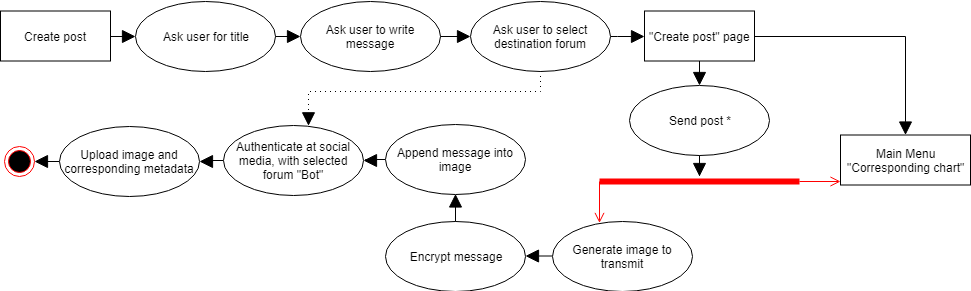
\includegraphics[width=0.95\textwidth]{Projectdoc/Assets/Illustrationer/Implementation-billede2.png}
    \label{fig:implementation2}
    \caption{Implementation 2}
\end{figure}

Gennem det 2. af 3 diagrammer beskrives både hvordan systemet håndterer at afsende en besked, jævnfør \ref{k:send}, men også hvad der videre kræves af brugeren for samme udførelse.\\
Brugeren bliver nemlig først promptet til, at skrive henholdsvis en titel for beskeden, herefter selve beskeden, og sidst at vælge et forum hvorunder beskeden hører til. Dette valgte forum får også senere betydning for beskedens uploads aktiviteter, da det bestemmer i hvilken sammenhæng beskeden skal findes, jævnfør \ref{k:sammen}, i denne demo også i direkte sammenhæng med en tilhørende bot, der agerer udgiver for de enkelte forums.\\
Hvis brugeren trykker på knappen \textit{post message}, vil systemet generere en asynkron tråd til at håndtere den videre udgivelse af brugerens besked, alt imens brugeren selv bliver omdirigeret til hovedmenuen.
Altså uden at brugeren bliver hindret, eller skal vente på at systemet generer et billede, jævnfør \ref{k:stegano}, indeholdende en krypteret version, af den ønskede besked, jævnfør \ref{k:krypto}. Systemet anvender tilsidst den valgte forum \textit{"bot"} til at udgive det færdig generede billede på det sociale medie, jævnfør \ref{k:lagre}.

\subsubsection{View posts}
\begin{figure}[H]
    \centering
    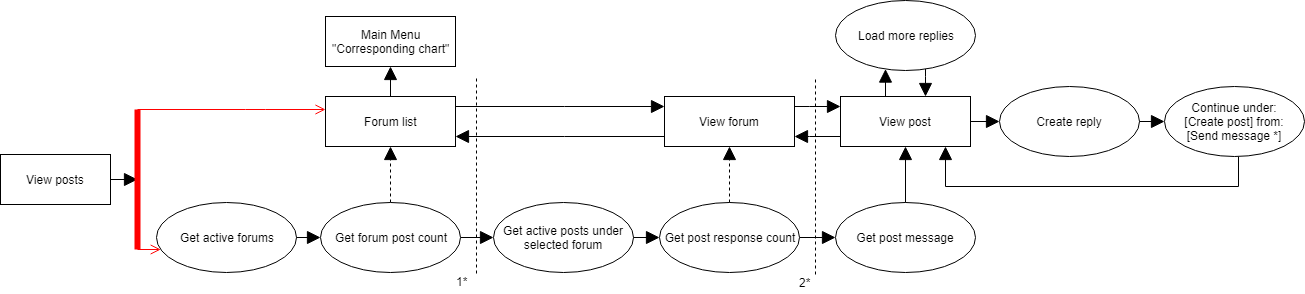
\includegraphics[width=1\textwidth, height=5cm]{Projectdoc/Assets/Illustrationer/Implementation-billede3.png}
    \label{fig:implementation3}
    \caption{Implementation 3}
\end{figure}

Gennem dette sidste diagram beskrives hvilke funktioner systemet anvender, under brugerens navigering af de allerede udgivne posts i de forskellige forums, udgivet gennem det anvendte sociale medie, jævnfør \ref{k:vise}.\\
Som ses i diagrammet splittes systemet nemlig allerede fra start til en asynkron tråd, der videre foretager de nødvendige baggrunds forespørgsler, for brugerens view. Dette er en praktisk anvendelse da brugeren så ikke oplever platformen som værende frosset i sine handlinger. Applikationen vil nemlig herved indeholde to aktive tråde, en til at fremvise resultater, og en til hentning af data, til alle tidspunkter.
F.eks. under første visning \textit{Forum List}, vil brugeren se en side med en roterende cirkel, symbolerende en load håndtering. Alt imens baggrundstråden foretager en række forespørgsler for hentning af de forskellige fora. Disse fora vil så, i takt med at de bliver hentet, videre blive præsenteret for brugeren i en liste der langsomt bliver udbygget, også medhjælpende til at udføre krav for indlæsnings tid, jævnfør \ref{k:load}.\\
Brugeren kan her, som eneste punkt, vælge at gå tilbage til hovedmenuen, eller fortsætte sin videre navigering, der efterfølgende også anvender den asynkrone baggrundstråd på samme måde som føromtalt.\\
Sidst hvis brugeren navigerer til en specifik besked, kan brugeren her også vælge at udfylde et nyt svar, der videre vil tage samme funktionalitet som før omtalt i 2. diagram \textit{Send Post}, under aktionen at brugeren har fuldført en besked, der videre sendes til det sociale medie.

\subsection{Brugergrænseflade}
\label{brugerflade}
Jævnfør \ref{k:naviger} og \ref{k:sikker} omhandlende henholdsvis krav om et intuitivt navigerbart system, og krav om tydelig identificerbar sikkerhed. Disse krav er grundstenene i systemets brugergrænse flade.\\
Der er mange elementer der spiller ind, når man snakker om at designe noget, der er intuitivt. I dette tilfælde handler det om, at skabe en platform som brugerne ikke skal tilvende sig til. Sagt med andre ord, skal platformen føles som en ganske almindelig moderne kommunikationsplatform i designet. Samtidig skal brugerne ikke være i tvivl om, at kommunikationen foregår anonymt, og uden ekstern overvågning. Ydermere adskiller platformen sig også i dets indhold, og ikke mindst i de brugere som platformen tiltrækker. Platformen er struktureret sådan for, at fremme meningsfulde debatter, og diskussioner omkring blandt andet teknologi og samfund. En af de strukturelle beslutninger, der er taget for at fremme netop denne form for indhold, er valg af forum struktur [Overvejelse fra system design \ref{forum_struktur}]. Der er i platformens struktur lagt indirekte vægt på, at brugerne tager sig mere tid til at skrive opslag, hvilket vil resultere i færre, men mere detaljeret opslag.

\subsubsection{Hovedmenu}
\begin{table}[H]
    \begin{minipage}{.5\textwidth}
        \begin{figure}[H]
            \centering
            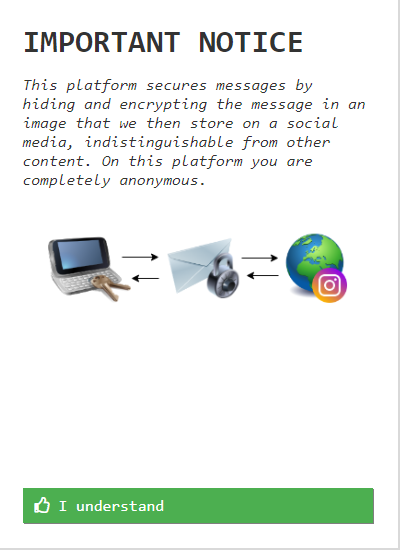
\includegraphics[width=0.90\linewidth]{Projectdoc/Assets/Illustrationer/splash.png}
            \caption{Varselsskærmen}
            \label{fig:splash}
        \end{figure}
    \end{minipage}
    \begin{minipage}{.5\textwidth}
        \begin{figure}[H]
            \centering
            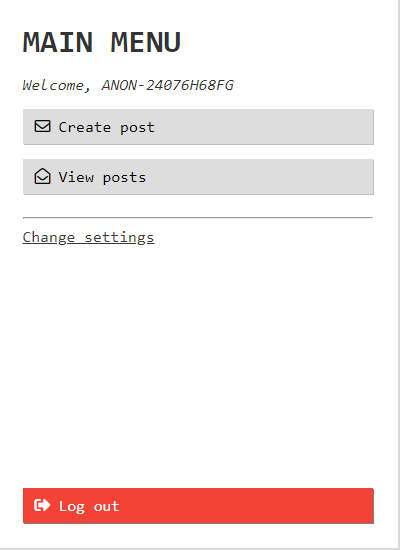
\includegraphics[width=0.90\linewidth]{Projectdoc/Assets/Illustrationer/main-menu.png}
            \caption{Hovedmenuen}
            \label{fig:mainmenu}
        \end{figure}
    \end{minipage}
\end{table}

Efter at brugeren succesfuldt er forbundet til bot netværket, vil brugeren blive mødt med følgende varsels skærm set på Figur \ref{fig:splash}. Denne varselsskærm har til formål at kort forklare hvordan platformen adskiller sig fra andre kommunikationsplatforme, og forklare brugerne at deres kommunikation er sikker. Denne varselsskærm vil kun blive vist ved første besøg i appen. Efter at brugeren tilkendegiver at have forstået indholdet af varselskærmen, anbringes brugeren direkte i hovedmenuen fra Figur \ref{fig:mainmenu}. Denne hovedmenu, består af et anonymt hash, navigation til menuerne: "Create post", "View posts" og "Change settings" og en log ud funktion. Det anonyme hash bliver genereret baseret på om, brugeren har autentificeret sig med det sociale medie eller ej. En uautentificeret bruger vil få et tilfældigt generet hash hver gang, mens en autentificeret bruger vil få et hash genereret ud fra vedkommendes bruger ID (fra det sociale medie). Denne sidst ville være nyttigt for brugere, der ønsker at kunne kædes sammen med tidligere opslag på platformen, for funktionaliteter så som sletning eller privat beskeder.

\subsubsection{Fora}
\begin{table}[H]
    \begin{minipage}{.33\textwidth}
        \begin{figure}[H]
            \centering
            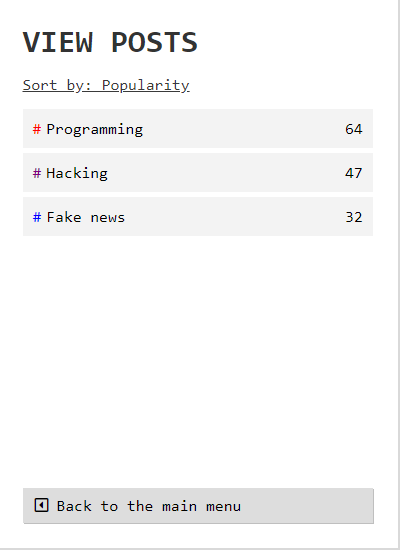
\includegraphics[width=0.95\linewidth]{Projectdoc/Assets/Illustrationer/forums.png}
            \caption{Forum oversigt}
            \label{fig:forum}
        \end{figure}
    \end{minipage}
    \begin{minipage}{.33\textwidth}
        \begin{figure}[H]
            \centering
            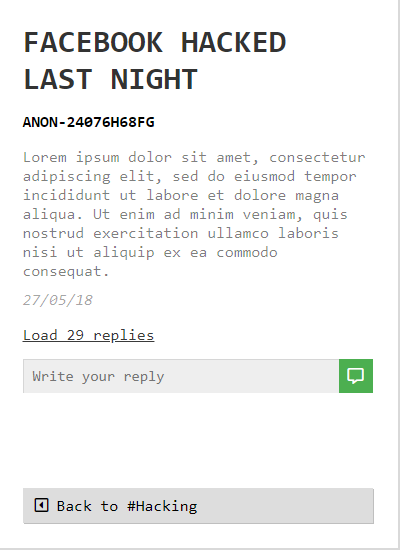
\includegraphics[width=0.95\linewidth]{Projectdoc/Assets/Illustrationer/post-inside.png}
            \caption{Indeni et opslag}
            \label{fig:mainpost}
        \end{figure}
    \end{minipage}
    \begin{minipage}{.33\textwidth}
        \begin{figure}[H]
            \centering
            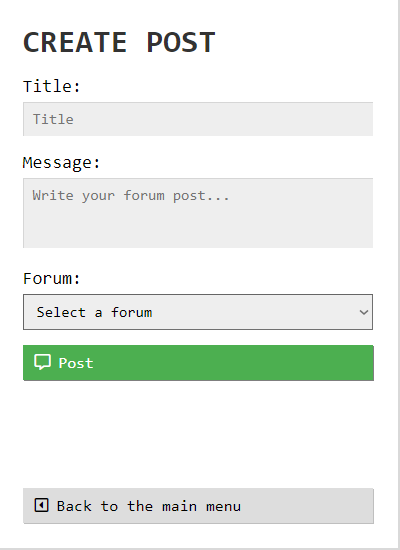
\includegraphics[width=0.95\linewidth]{Projectdoc/Assets/Illustrationer/send.png}
            \caption{Opret opslag}
            \label{fig:sendpost}
        \end{figure}
    \end{minipage}
\end{table}

Hvis brugeren ønsker at gennemse opslag lavet af andre brugere, navigerer de sig hen til forums oversigten, vist ved Figur \ref{fig:forum}. Denne oversigt indeholder alle tilgængelige fora på platformen. Tallet til højre for navnet på forumet, beskriver hvor mange aktive tråde forumet har på et givet tidspunkt. Hvis brugeren navigerer sig ind på et forum, vil brugeren blive præsenteret for en lignede oversigt, denne gang bare med forumets individuelle opslag. Brugeren vælger her et opslag, og bliver præsenteret for en side som på Figur \ref{fig:mainpost}. Dette er layoutet for alle opslag. Opslaget består af: titlen, bruger-hashet, beskeden, en dato, og et kommentarfelt. Kommentarerne på opslaget er ikke indlæst som standard, for at undgå for mange unyttige forespørgsler, både for brugeren, men også for selve systemet og det sikkerhed.\\
Brugeren kan også vælge at oprette en tråd/opslag på et forum, ved at navigere sig hen til "Create post" i hovedmenuen. Siden viser de tre inputs: titel, besked og destinations forum, der alle skal udfyldes for at oprette en ny tråd, vist ved Figur \ref{fig:sendpost}.